% Measured Analysis figures, generated 2026-11-16.
% Requires graphicx. Put this in the preamble (relative to your paper root):
% \graphicspath{{paper_assets/acd_figures/analysis_20261116/}}
% Alternatively copy the PDFs into figs/ and adapt the paths.
% Select the relevant environments; including all ten is not a main-paper recommendation.
% Pilot, historical endpoint, and post-hoc evidence must retain their scope labels.

\begin{figure*}[t]
  \centering
  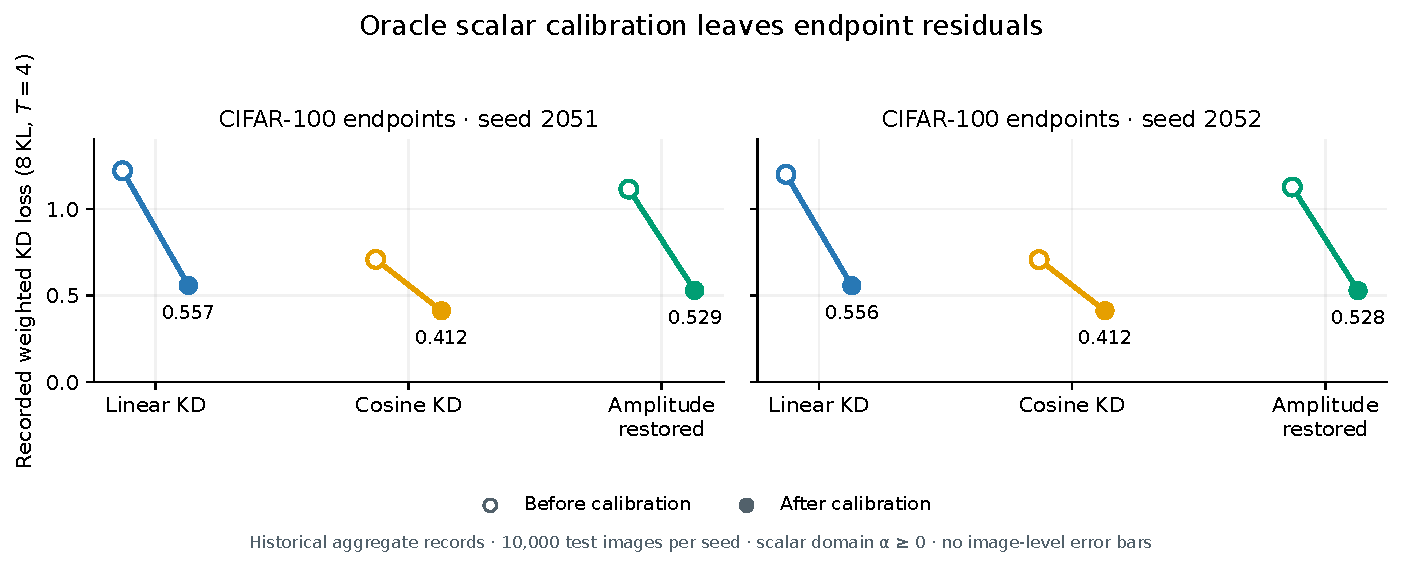
\includegraphics[width=0.92\textwidth]{fig_oracle_calib.pdf}
  \caption{\textbf{Oracle scalar calibration of historical CIFAR-100 endpoints.}
  Open and filled markers show the recorded mean distillation loss before and
  after per-image scalar calibration on all 10,000 test images, respectively.
  Each panel reports a separate training seed. The recorded objective is
  $8\,\mathrm{KL}(p_T\|q_T)$ at $T=4$; calibration minimizes it over a multiplier
  $\alpha\geq0$ applied to the entire student logit vector. The boundary
  $\alpha=0$ represents the infimum over strictly positive multipliers.
  Cosine-trained endpoints have lower residuals in these records, but the
  comparison does not isolate an immediate coordinate-substitution effect.
  The plot is reconstructed from saved aggregate summaries, without
  image-level uncertainty estimates; these models do not constitute an ETF ablation.}
  \label{fig:oracle_calib}
\end{figure*}

\begin{figure*}[t]
  \centering
  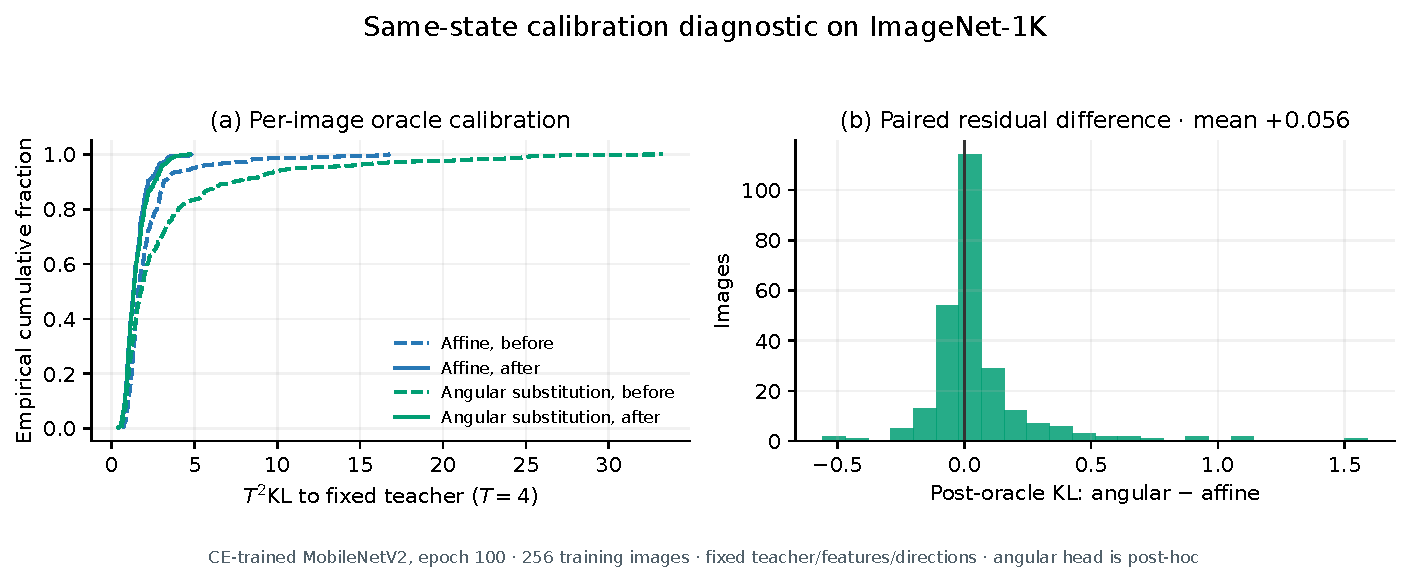
\includegraphics[width=0.92\textwidth]{fig_oracle_same_state.pdf}
  \caption{\textbf{Same-state calibration diagnostic on ImageNet-1K.}
  We fix an epoch-100 CE-trained MobileNetV2, its features and classifier
  directions, an official ResNet50 teacher, and 256 preselected training images.
  The original affine head is compared with the post-hoc angular head
  $z_k=30\cos\theta_k$. Left: empirical distributions of
  $T^2\mathrm{KL}(p_T\|q_T)$, $T=4$, before and after independent per-image
  oracle calibration over $\alpha\geq0$. Right: paired post-oracle residual
  differences, angular minus affine. The mean difference is $+0.0563$
  (affine $1.4742$, angular $1.5305$). Direct angular substitution therefore
  does not reduce the mean residual in this diagnostic. This experiment
  does not evaluate a student trained with ACI.}
  \label{fig:oracle_same_state}
\end{figure*}

\begin{figure*}[t]
  \centering
  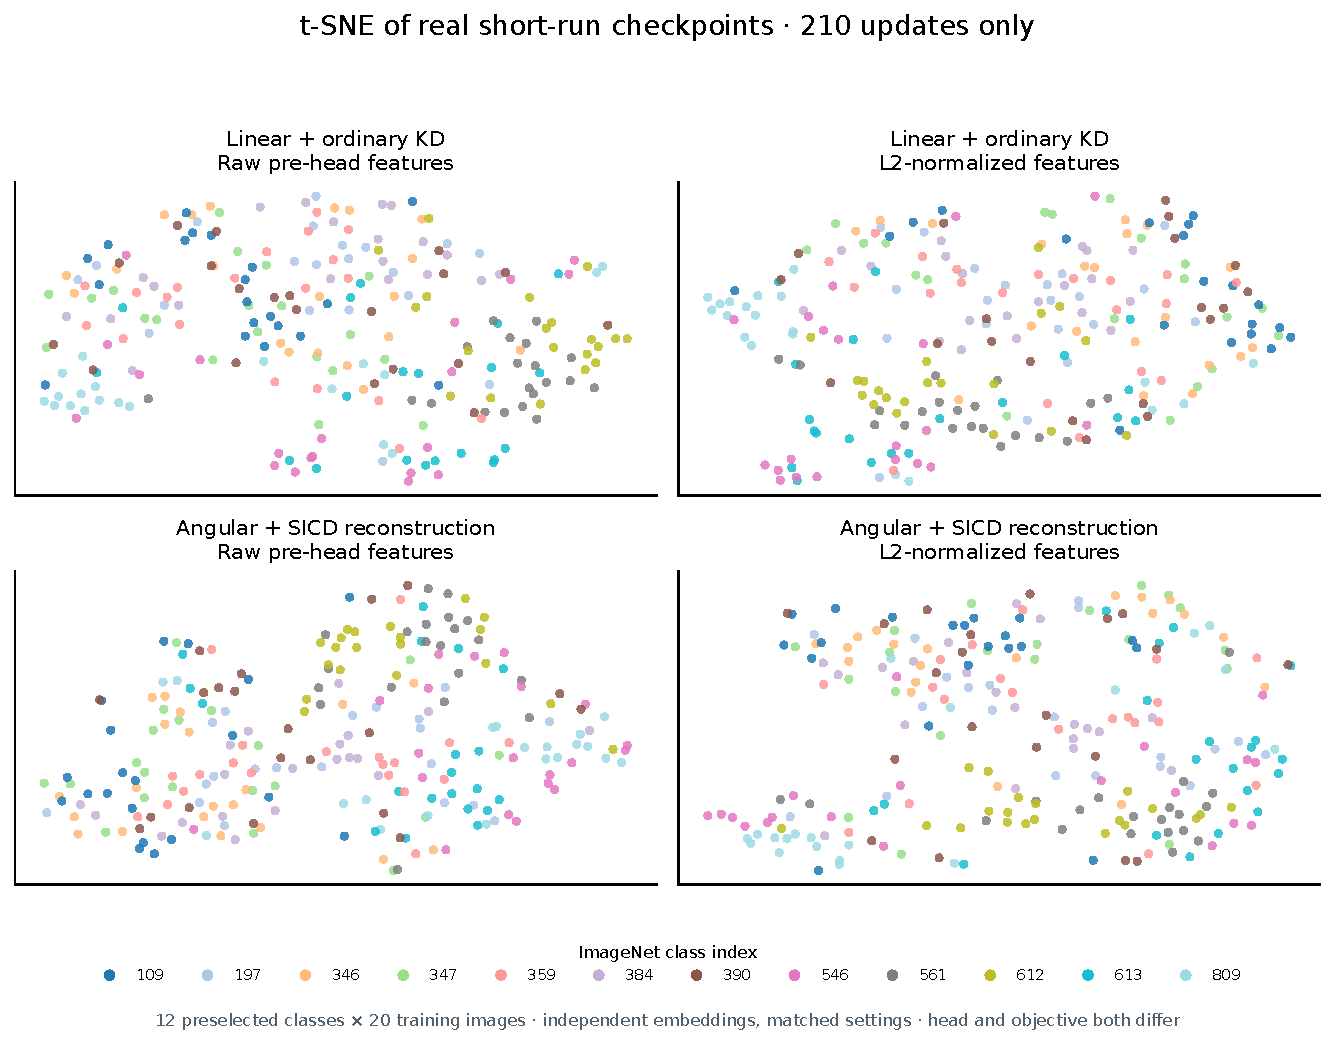
\includegraphics[width=0.85\textwidth]{fig_tsne_pilot.pdf}
  \caption{\textbf{Qualitative representation diagnostic of 210-update pilots.}
  Rows compare a linear-head KD pilot with an angular-head pilot using the
  SICD equation reconstruction. Columns use raw pre-head features and their
  L2-normalized counterparts. All panels use the same 240 ImageNet training
  images from 12 preselected classes, identical initial two-dimensional
  coordinates, perplexity 30, random seed 7, and 1,000 t-SNE iterations.
  Colors denote classes. Each panel is fitted independently, so plot
  orientation, scale, and inter-cluster distances are not directly comparable.
  Both head and training objective differ between rows; the pilots use
  no ETF initialization and do not establish an isolated ACI effect,
  final representation quality, or alignment with teacher semantics.}
  \label{fig:tsne}
\end{figure*}

\begin{figure*}[t]
  \centering
  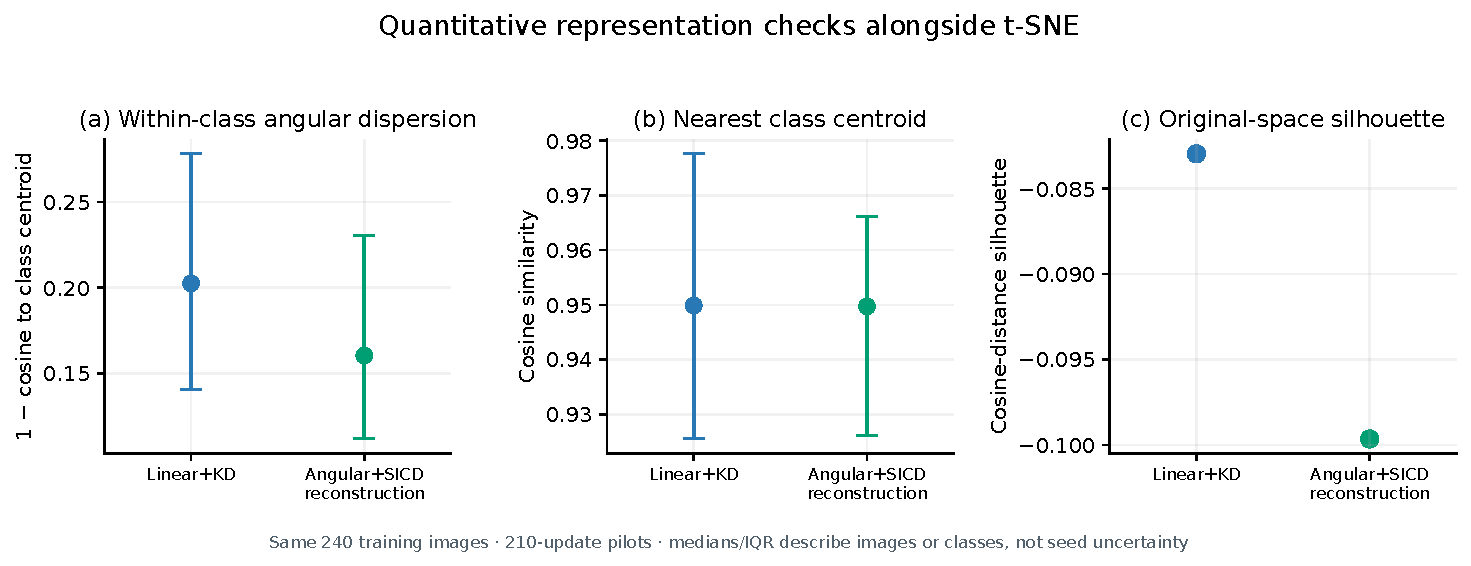
\includegraphics[width=0.95\textwidth]{fig_representation_pilot.pdf}
  \caption{\textbf{Original-space checks accompanying the pilot t-SNE.}
  On the same 240 images, we measure cosine distance to each sample's
  normalized class centroid, cosine similarity to the nearest other class
  centroid, and cosine-distance silhouette in the original feature space.
  For the first two panels, dots and bars denote medians and interquartile
  ranges over images and classes, respectively; they are not confidence
  intervals over independent training seeds. The angular/SICD reconstruction
  pilot has lower within-class dispersion but a lower silhouette score.
  These mixed short-run findings do not establish uniformly better class separation.}
  \label{fig:representation_metrics}
\end{figure*}

\begin{figure*}[t]
  \centering
  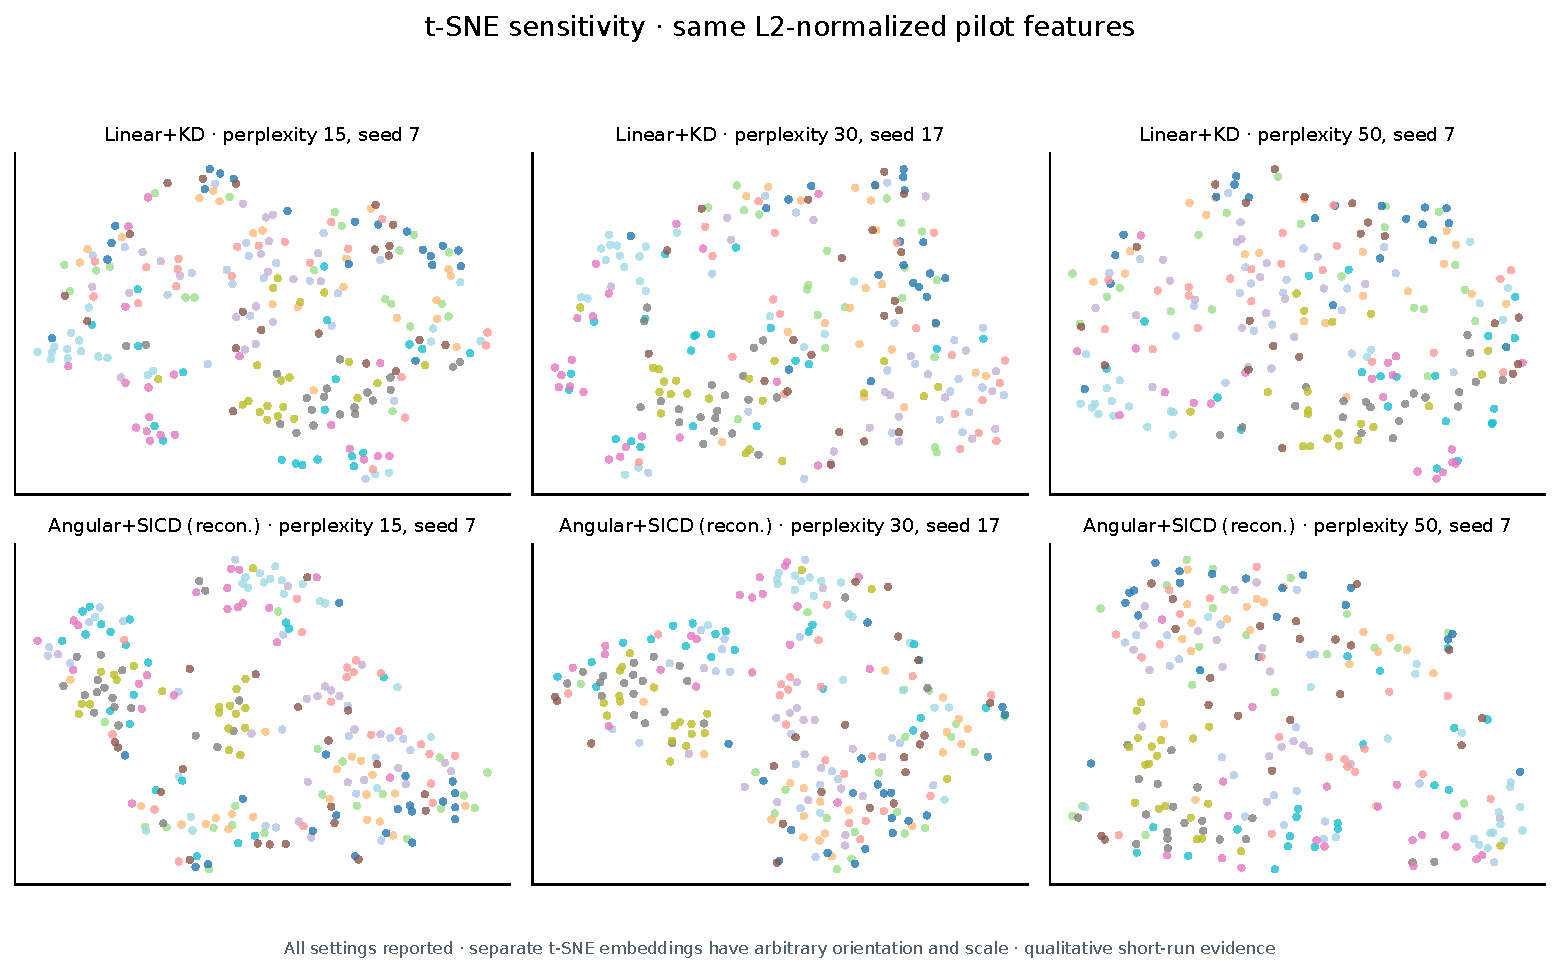
\includegraphics[width=0.95\textwidth]{fig_tsne_sensitivity.pdf}
  \caption{\textbf{Sensitivity of the pilot t-SNE visualization.}
  We repeat the embedding of the same L2-normalized pilot features with
  $(\mathrm{perplexity},\mathrm{seed})$ equal to $(15,7)$, $(30,17)$, and $(50,7)$.
  All tested additional settings are shown; this is not an exhaustive grid.
  Images, labels, and colors match Fig.~\ref{fig:tsne}. Layout variation
  motivates interpreting t-SNE together with the original-space measurements
  in Fig.~\ref{fig:representation_metrics}.}
  \label{fig:tsne_sensitivity}
\end{figure*}

\begin{figure*}[t]
  \centering
  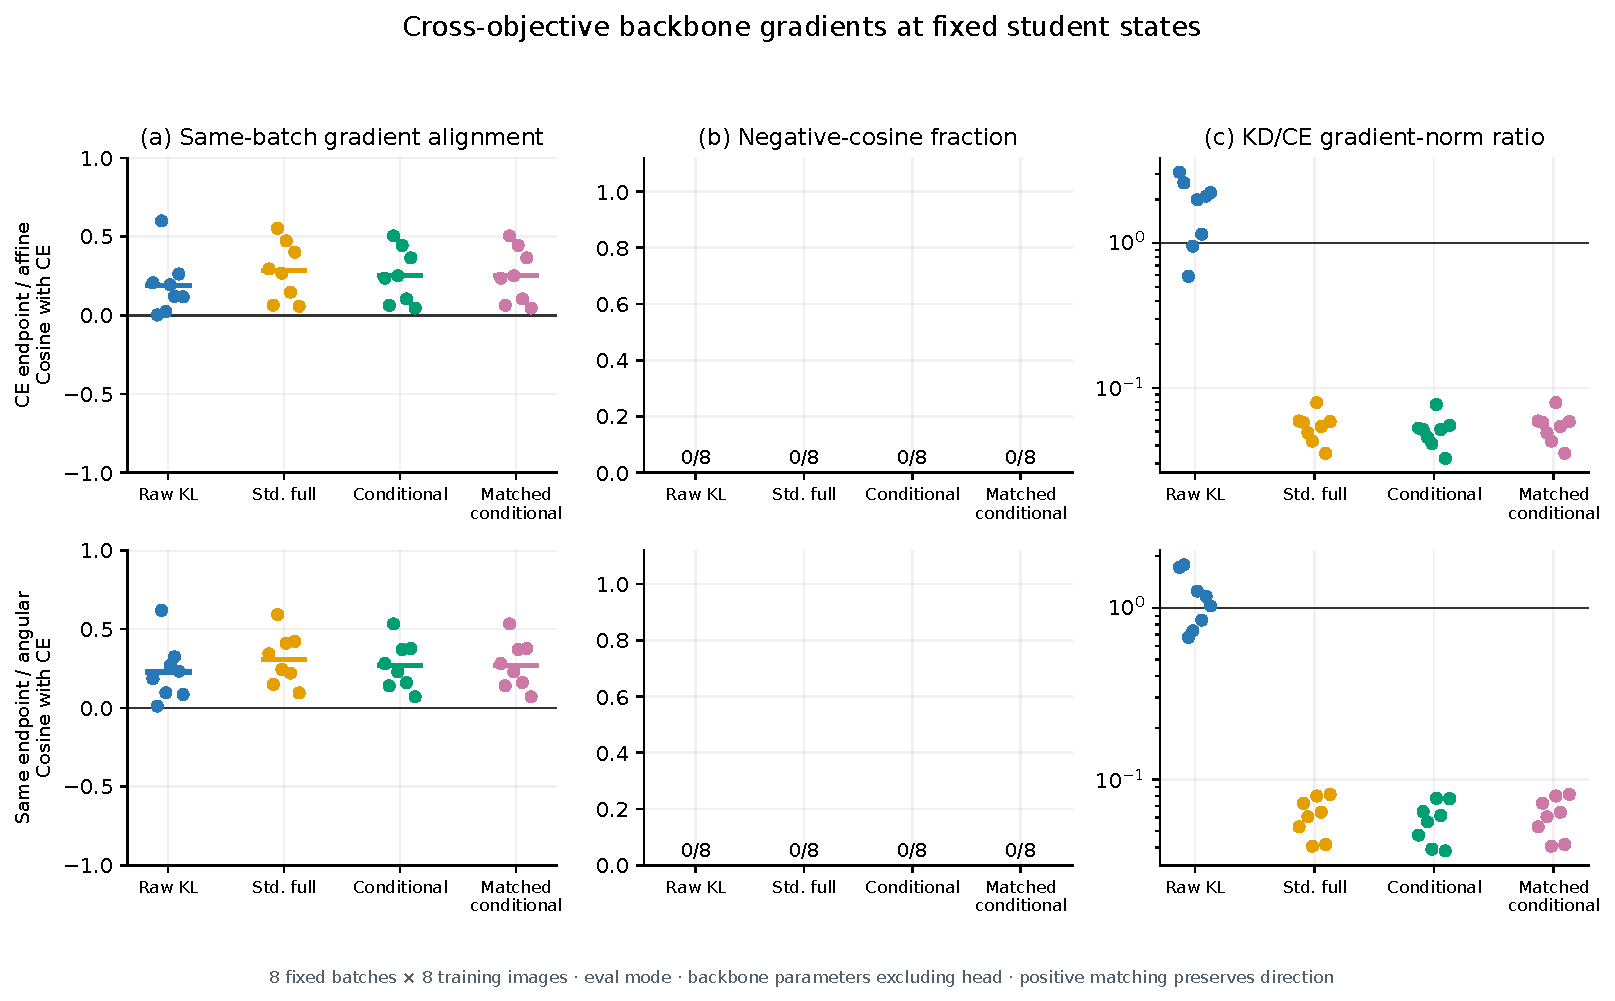
\includegraphics[width=0.95\textwidth]{fig_gradient_conflict.pdf}
  \caption{\textbf{Same-batch CE--distillation gradient diagnostics.}
  Rows use a CE-trained epoch-100 MobileNetV2 with its original affine head
  and the same endpoint with a post-hoc angular head. Within each state,
  we evaluate raw KL, dual-side standardized full KL, teacher-mass-weighted
  standardized conditional KL, and positively norm-matched conditional KL
  on eight fixed batches of eight ImageNet training images at $T=4$.
  Gradients concatenate all trainable backbone parameters excluding the head;
  batch normalization is frozen and dropout disabled. Panels show CE cosine
  similarity, negative-cosine batch fraction, and KD-to-CE norm ratio.
  Matching targets the standardized-full backbone gradient norm and preserves
  conditional gradient direction. All objectives have zero negative-cosine
  batches in this sample. These fixed-state results do not demonstrate
  elimination of training-time gradient conflicts.}
  \label{fig:gradient_conflict}
\end{figure*}

\begin{figure*}[t]
  \centering
  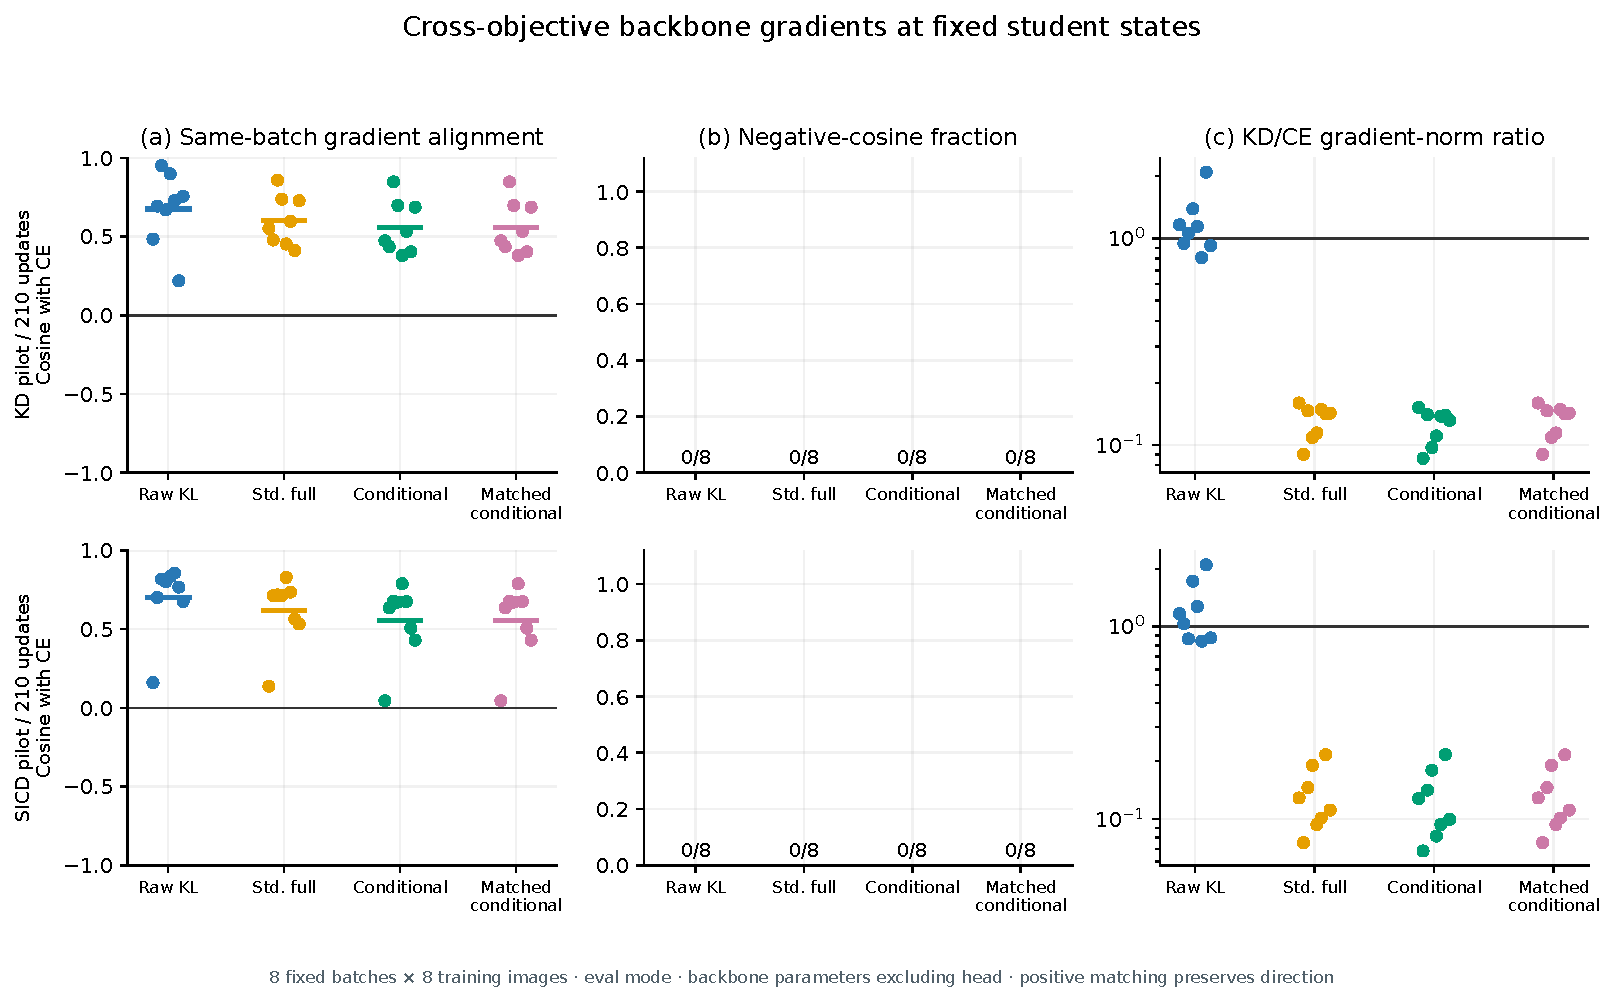
\includegraphics[width=0.95\textwidth]{fig_gradient_conflict_pilot.pdf}
  \caption{\textbf{Gradient diagnostics at real short-run pilot states.}
  We apply the same batches, objectives, parameter set, evaluation mode,
  and norm-matching convention as Fig.~\ref{fig:gradient_conflict} to the
  linear/KD and angular/SICD-reconstruction checkpoints after 210 updates.
  No measured objective has a negative CE cosine on these eight batches;
  conditional supervision does not consistently improve CE alignment.
  These are local measurements, not full-training trajectories or
  independent-seed estimates of optimization behavior.}
  \label{fig:gradient_conflict_pilot}
\end{figure*}

\begin{figure*}[t]
  \centering
  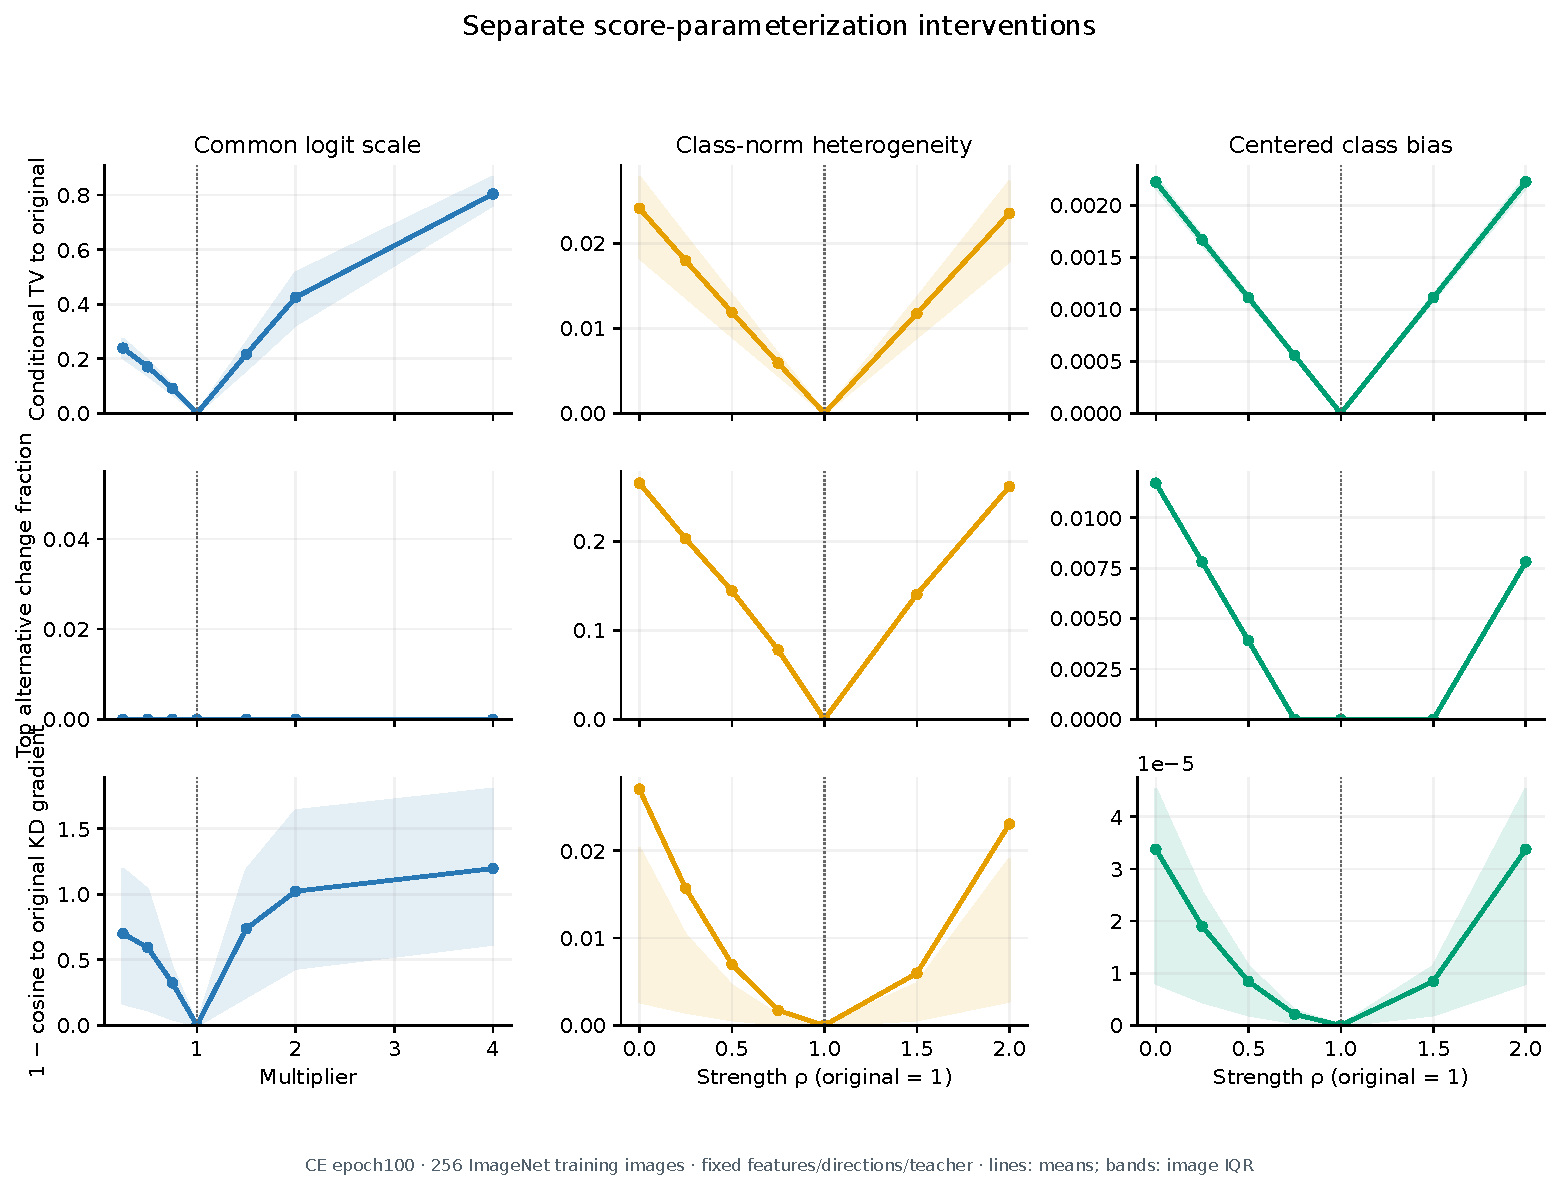
\includegraphics[width=0.95\textwidth]{fig_parameterization.pdf}
  \caption{\textbf{Separate interventions on score parameterization.}
  We fix the epoch-100 CE student features, classifier directions,
  ResNet50 teacher outputs, and 256 ImageNet training images. Columns vary
  the multiplier of the entire logit vector; class-weight norm heterogeneity,
  $n_k(\rho)=\bar n_g\exp(\rho\log(n_k/\bar n_g))$, with $\bar n_g$ the
  geometric mean; and centered class bias,
  $b_k(\rho)=\bar b+\rho(b_k-\bar b)$. The original model is recovered at 1.
  Rows show non-target conditional total variation at $T=4$, the fraction
  whose highest-scoring non-target class changes, and feature-gradient
  direction deviation from the original full-KL gradient.
  Lines denote means and shaded regions image interquartile ranges.
  Positive common scaling preserves rankings, whereas class-dependent
  factors can alter them. Intervention ranges are not matched by a common
  perturbation norm and do not establish relative causal importance.}
  \label{fig:parameterization_factors}
\end{figure*}

\begin{figure*}[t]
  \centering
  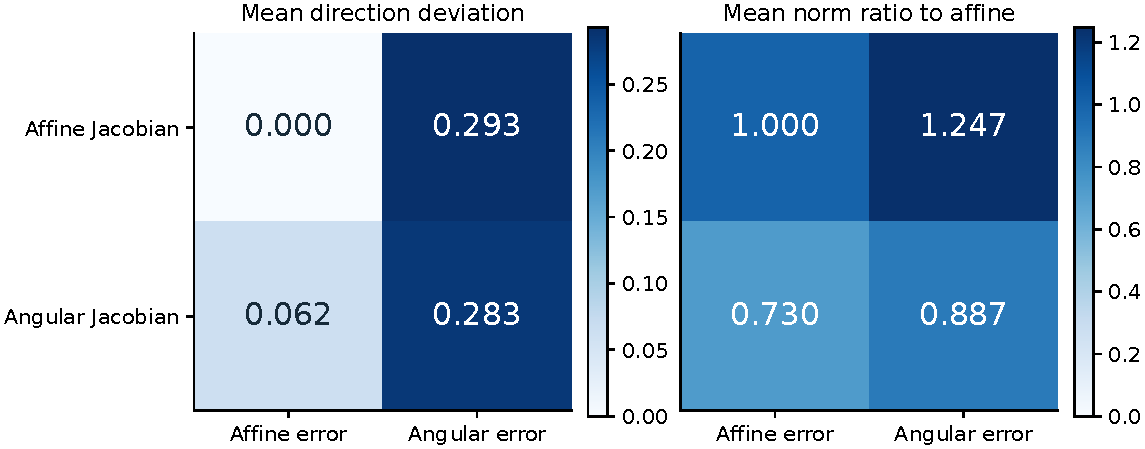
\includegraphics[width=0.9\textwidth]{fig_gradient_sources.pdf}
  \caption{\textbf{Probability-error and Jacobian contributions to local gradients.}
  With fixed student features, classifier directions and teacher outputs,
  we form $g=J^\top T(q_T-p_T)$ using the affine or angular classifier
  Jacobian and the affine or angular student probability error.
  The reference is the original affine/affine feature gradient.
  Heatmaps show mean direction deviation $1-\cos(g,g_{\mathrm{ref}})$
  and norm ratio over 256 ImageNet training images.
  Crossed cells are constructed diagnostic vectors, not gradients of an
  evaluated training pipeline. Both paths alter local gradients; the cells
  should not be interpreted as additive causal contributions or accuracy gains.}
  \label{fig:gradient_sources}
\end{figure*}

\begin{figure*}[t]
  \centering
  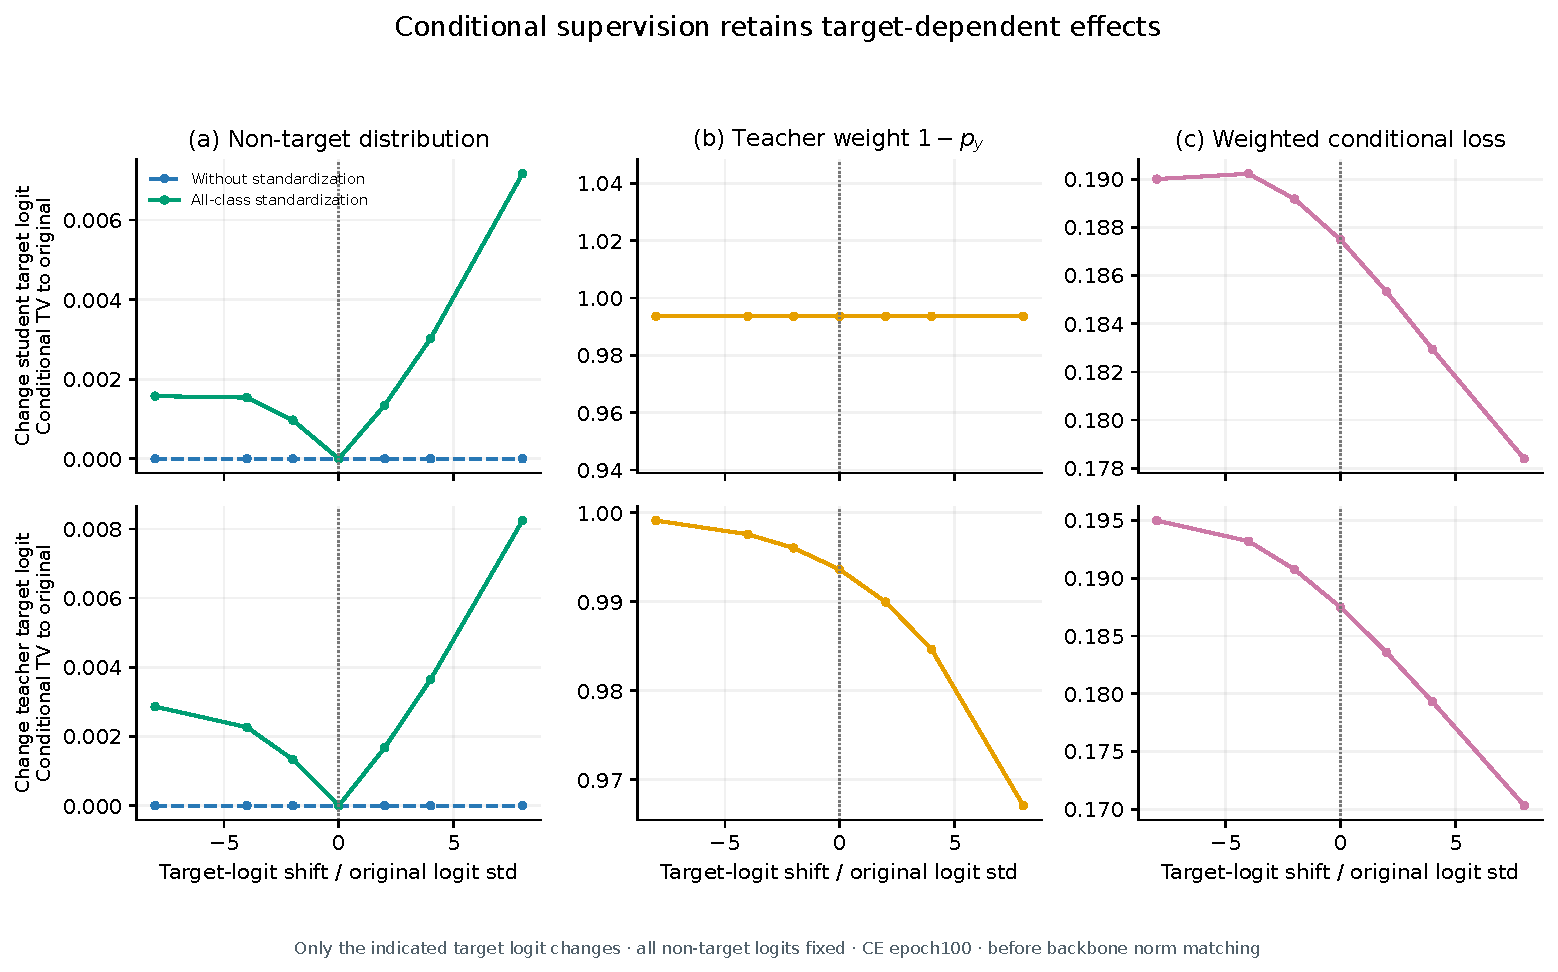
\includegraphics[width=0.95\textwidth]{fig_conditional_dependency.pdf}
  \caption{\textbf{Target-logit dependence remaining in conditional supervision.}
  On 256 fixed ImageNet training images, we shift only the student target
  logit (top) or teacher target logit (bottom), in units of that image's
  original logit standard deviation; all non-target logits remain fixed.
  Left: mean non-target conditional TV from the unperturbed distribution,
  with and without all-class standardization. Middle: mean teacher
  non-target mass $1-p_y$ after standardization. Right: mean
  $(1-p_y)T^2\mathrm{KL}(p_{\neg y}\|q_{\neg y})$, $T=4$,
  before backbone norm matching. Removing the explicit binary target-mass
  KL term does not remove dependence through all-class standard deviation
  or teacher weighting. Unstandardized conditional distributions remain
  exactly unchanged under these target-only interventions.}
  \label{fig:conditional_dependency}
\end{figure*}
